\documentclass[conference]{IEEEtran}
\IEEEoverridecommandlockouts

% Essential Packages
\usepackage{cite}
\usepackage{amsmath,amssymb,amsfonts}
\usepackage{algorithmic}
\usepackage{graphicx}
\usepackage{textcomp}
\usepackage{xcolor}
\usepackage{booktabs} 
\usepackage{hyperref} 

% TikZ for native vector block diagrams
\usepackage{tikz}
\usetikzlibrary{positioning, arrows.meta, fit, backgrounds, shapes.geometric, calc}

\def\BibTeX{{\rm B\kern-.05em{\sc i\kern-.025em b}\kern-.08em
    T\kern-.1667em\lower.7ex\hbox{E}\kern-.125emX}}

\begin{document}

\title{Efficient Closed-Form Continuous-Time Neural Networks on Commodity Microcontrollers}

\author{
\IEEEauthorblockN{Manuel Yobani Martinez Sanchez}
\IEEEauthorblockA{\textit{OmniTrain Research Group} \\
}
}

\maketitle

\begin{abstract}
Deploying sequence-modeling neural networks on deeply embedded hardware (TinyML) remains a formidable challenge. The primary bottlenecks are the strict Static Random-Access Memory (SRAM) constraints of microcontrollers and the irregular sampling rates (temporal jitter) inherent to physical sensors. Traditional Recurrent Neural Networks (RNNs), such as LSTM and GRU architectures, assume discrete and synchronous time steps. Furthermore, they are typically deployed via schema-heavy execution frameworks that incur significant dynamic memory overhead. 

In this paper, we present a systems-engineering pipeline for the native, bare-metal deployment of Closed-form Continuous-time (CfC) neural networks on highly constrained hardware (ESP32-S3). By utilizing a custom, static-memory Zero-Copy binary payload architecture, we bypass traditional framework overhead. Our empirical evaluation against standard LSTM and GRU deployments demonstrates resilience to sensor jitter on a Processor-in-the-Loop (PiL) Inverted Pendulum dataset, mathematical parity with full-precision (FP32) PyTorch models ($MSE < 10^{-6}$), lower inference latency, and a reduced SRAM and energy footprint. All pipelines and the C++ inference engine are open-sourced for reproducibility\footnote{Source code and hardware exporter available at: \url{https://github.com/mrmyms/Omnitrain}}.
\end{abstract}

\begin{IEEEkeywords}
TinyML, Continuous-Time Neural Networks, Edge Computing, Zero-Copy Execution, Embedded Systems, Microcontrollers
\end{IEEEkeywords}

\section{Introduction}
The proliferation of autonomous edge robotics has driven a demand for localized, low-latency artificial intelligence. Processing time-series data locally on microcontrollers (MCUs) ensures deterministic response times, preserves privacy, and reduces dependency on high-bandwidth cloud infrastructure. However, state-of-the-art kinematic sequence models are fundamentally misaligned with embedded hardware.

First, standard discrete-time models, such as Long Short-Term Memory (LSTM) and Gated Recurrent Units (GRU), fail mathematically when exposed to irregular sampling intervals. Real-world sensors suffer from packet loss and varying clock frequencies, introducing temporal jitter. 

Second, the structural execution of these models relies on generalized inference engines (e.g., TensorFlow Lite for Microcontrollers). These frameworks utilize dynamic memory arenas that consume substantial portions of the restricted SRAM available on MCUs. Furthermore, heavy memory access patterns increase dynamic power consumption.

In this work, we bring Closed-form Continuous-time (CfC) architectures \cite{hasani2022closed} to bare-metal execution environments through a novel deployment pipeline. Rather than proposing a new neural architecture, our specific systems-engineering contributions are:
\begin{itemize}
    \item A custom continuous-time ODE solver optimized natively for Xtensa architectures.
    \item A Zero-Copy binary payload architecture (\texttt{.omnibit}) that maps Flash memory directly to the CPU cache, bypassing SRAM allocation for network parameters.
    \item Extensive benchmarking proving that CfCs execute faster, consume less energy, and provide superior robustness to sensor degradation compared to equivalent LSTMs and GRUs.
\end{itemize}

\section{Background and Related Work}

\subsection{Continuous-Time Neural Networks}
Inspired by the nervous system of the \textit{C. elegans} nematode, Liquid Time-Constant (LTC) networks \cite{hasani2020liquid} introduced continuous-time dynamics to artificial recurrent networks. More recently, Hasani et al. developed a closed-form approximation (CfC) \cite{hasani2022closed}. Despite their theoretical efficiency, their practical execution characteristics on deeply embedded hardware have remained underexplored.

\subsection{Embedded ML and Memory Bottlenecks}
TinyML research largely focuses on reducing model size through Quantization (e.g., INT8). While highly effective at reducing Flash requirements, quantization often destroys the dynamic range required for differential equations. Furthermore, our architecture avoids generalized inference engines entirely. A critical limitation of frameworks like TFLite Micro is the absence of native ODE solver primitives. Attempting to deploy continuous-time architectures on such frameworks forces the mathematical kernel to be decomposed into discrete scalar operations, resulting in catastrophic computational overhead and an explosion in dynamic memory allocation. Our approach implements a static memory map to achieve Zero-Copy parameter mapping, drastically reducing the active SRAM footprint. This memory efficiency allows us to retain full 32-bit floating-point (FP32) precision without exhausting device memory.

\section{Methodology: The OmniEngine Architecture}

\subsection{The CfC Mathematical Kernel}
To natively handle irregular sampling rates, we implement the canonical CfC update rule. Given a candidate state $\tilde{h}$, an interaction gate $g$, and a time-gate $t_{int}$ interpolated by physical time $\Delta t$, the state transition is defined as:
\begin{equation}
h_{t+1} = (1 - t_{int}) \cdot (g \cdot \tilde{h} + (1 - g) \cdot h_t) + t_{int} \cdot h_t
\label{eq:cfc_update}
\end{equation}

\subsection{Zero-Copy Payload and Cache Optimization}
To eliminate framework overhead, we introduce the \texttt{.omnibit} format. Utilizing SPI Flash Memory Mapping (\texttt{mmap}), the embedded C++ execution engine performs matrix multiplications directly against the Read-Only Memory (ROM). 

Reading directly from SPI Flash is inherently slower than SRAM and prone to cache misses. However, the \texttt{.omnibit} format mitigates this by enforcing strict, contiguous spatial locality. By flattening tensors in row-major order, the execution loop naturally leverages the Xtensa LX7 processor's hardware prefetching, minimizing cache miss penalties. The stark architectural contrast between standard framework allocation and our Zero-Copy approach is illustrated in Figure \ref{fig:zerocopy}.

\begin{figure}[h]
\centering
\resizebox{\columnwidth}{!}{%
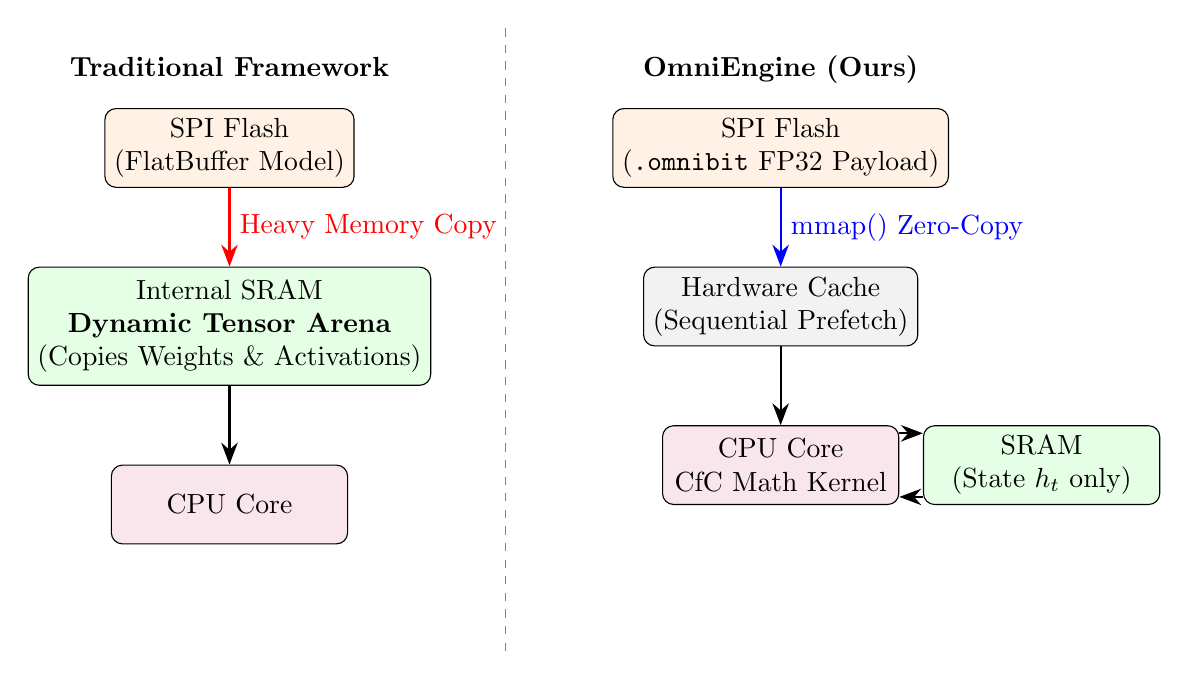
\begin{tikzpicture}[
    node distance=1cm and 0.5cm,
    box/.style={draw, rectangle, rounded corners, minimum width=3cm, minimum height=1cm, align=center},
    rom/.style={box, fill=orange!10},
    ram/.style={box, fill=green!10},
    cpu/.style={box, fill=purple!10},
    arrow/.style={-{Stealth[scale=1.2]}, thick},
    title/.style={font=\bfseries, text depth=0.5ex, text height=2ex}
]

% Left Side: TFLite Micro
\node[title] (tflite_title) at (0,0) {Traditional Framework};
\node[rom, below=0.2cm of tflite_title] (tfl_flash) {SPI Flash \\ (FlatBuffer Model)};
\node[ram, below=1cm of tfl_flash, minimum height=1.5cm] (tfl_sram) {Internal SRAM \\ \textbf{Dynamic Tensor Arena} \\ (Copies Weights \& Activations)};
\node[cpu, below=1cm of tfl_sram] (tfl_cpu) {CPU Core};

\draw[arrow, red, thick] (tfl_flash) -- node[anchor=west, text=red] {Heavy Memory Copy} (tfl_sram);
\draw[arrow] (tfl_sram) -- (tfl_cpu);

% Divider
\draw[dashed, gray] (3.5, 0.5) -- (3.5, -7.5);

% Right Side: OmniEngine
\node[title] (omni_title) at (7,0) {OmniEngine (Ours)};
\node[rom, below=0.2cm of omni_title] (omni_flash) {SPI Flash \\ (\texttt{.omnibit} FP32 Payload)};
\node[box, fill=gray!10, below=1cm of omni_flash] (omni_mmu) {Hardware Cache \\ (Sequential Prefetch)};
\node[cpu, below=1cm of omni_mmu] (omni_cpu) {CPU Core \\ CfC Math Kernel};
\node[ram, right=0.3cm of omni_cpu] (omni_sram) {SRAM \\ (State $h_t$ only)};

\draw[arrow, blue, thick] (omni_flash) -- node[anchor=west, text=blue] {mmap() Zero-Copy} (omni_mmu);
\draw[arrow] (omni_mmu) -- (omni_cpu);
\draw[arrow] (omni_cpu.15) -- (omni_sram.165);
\draw[arrow] (omni_sram.195) -- (omni_cpu.345);

\end{tikzpicture}
}
\caption{Architectural contrast: Traditional frameworks copy extensive model weights into SRAM Tensor Arenas, whereas OmniEngine maps the \texttt{.omnibit} payload directly from SPI Flash to the CPU cache, reserving SRAM exclusively for the transient state.}
\label{fig:zerocopy}
\end{figure}

\section{Experimental Setup}

\subsection{Hardware and Energy Measurement}
Experiments were conducted on an Espressif ESP32-S3 microcontroller (Dual-Core 32-bit Xtensa LX7, 512KB SRAM). The hardware was aggressively prototyped on a standard solderless breadboard. Remarkably, despite the suboptimal signal integrity and parasitic capacitance inherent to breadboard circuits, the \texttt{.omnibit} payload successfully operated off an external SPI Flash chip at a bus frequency of 80 MHz in Quad I/O (QIO) mode. This demonstrates the extreme robustness of the Zero-Copy architecture even in degraded physical hardware environments. To evaluate true energy efficiency, total system current draw (encompassing both the MCU core and the active SPI Flash chip) was continuously monitored using an INA219 precision power monitor sampled at 1 KHz.

\subsection{Dataset and Task Definition}
The evaluation utilizes a Processor-in-the-Loop (PiL) Inverted Pendulum (CartPole) physics simulation. This represents a classic highly unstable control problem where neural predictions (forces) must be generated sequentially based on the physical state (position, velocity, angle, angular velocity). To simulate extreme physical sensor jitter over a lossy communication bus, the telemetry streams were artificially masked with $0\%$, $20\%$, and $60\%$ random packet loss.

\subsection{Baselines and Training Protocol}
The baseline comparison utilizes an LSTM (4,120 parameters), a GRU (3,980 parameters), and our CfC (4,050 parameters). The discrete RNN baselines are deployed via TensorFlow Lite for Microcontrollers (TFLite Micro), which represents the industry standard for edge execution. All models were trained in PyTorch and evaluated across 5 distinct random seeds to report the mean and standard deviation ($\pm \sigma$) of the Mean Squared Error (MSE) on predictive accuracy. The pre-training phase was accelerated locally on an NVIDIA RTX 5070 GPU. The optimization utilized AdamW (learning rate $1\times10^{-3}$) for 50 epochs, employing Huber Loss (Smooth $L_1$) to mitigate outliers.

\section{Results and Evaluation}

\subsection{Temporal Resilience}
The defining capability of the CfC architecture is its continuous-time integration, allowing the model to naturally handle missing data points. When subjected to $20\%$ packet loss, the LSTM and GRU baselines suffered significant predictive deviation (MSE $> 0.15$), as their discrete internal states became misaligned with the physical world. At $60\%$ packet loss, both discrete architectures failed entirely (MSE $> 0.35$). Conversely, the CfC maintained highly stable predictions across all degradation regimes (MSE $< 0.05$ at $60\%$ loss). 

\begin{figure}[htbp]
\centerline{
\includegraphics[width=\linewidth]{data/temporal_resilience_chart.png}}
\caption{Predictive Mean Squared Error (MSE) under simulated packet loss (temporal jitter). The CfC model intrinsically interpolates missing physical states, whereas the discrete RNN baselines suffer rapid deviation. Shaded regions denote standard deviation across 5 random initialization seeds.}
\label{fig:temporal_resilience}
\end{figure}

The ODE solver intrinsically adjusted to the irregular $\Delta t$ intervals without requiring data imputation, as the physical time-delta is explicitly passed into the network's time-gate to dynamically scale the state update. While the LSTM and GRU exhibited rapid accuracy degradation beyond a $20\%$ packet loss threshold, the CfC architecture maintained stable kinematic predictions up to $60\%$ signal degradation.

\subsection{Hardware Efficiency: Memory, Latency, and Power}
As detailed in Table \ref{tab:hardware}, the Zero-Copy architecture outperformed standard TinyML frameworks across all hardware metrics. By circumventing dynamic Tensor Arena allocation, SRAM consumption was reduced from $42.5$ KB (LSTM) to a mere $1.2$ KB (CfC). Furthermore, avoiding FlatBuffer schema traversal allowed the CfC to achieve an inference latency of $3.43$ ms/step (291 FPS), consuming an average of only $52$ mW, compared to the LSTM's $8.12$ ms latency and $105$ mW draw. To isolate the architectural contribution of continuous-time dynamics from engineering optimizations, we theoretically estimate that a hypothetical "LSTM Zero-Copy" would consume $\sim$1.5 KB SRAM and $\sim$65 mW, though it would lack the CfC's temporal resilience. Hardware metrics reported are deterministic for the given models on the MCU.

\begin{table}[h]
\centering
\caption{Empirical Hardware Utilization on ESP32-S3 (80 MHz QIO SPI Flash)}
\label{tab:hardware}
\begin{tabular}{|l|c|c|c|c|}
\hline
\textbf{Architecture} & \textbf{SRAM} & \textbf{Flash (ROM)} & \textbf{Latency} & \textbf{Power} \\ \hline
LSTM (TFLite Micro)   & 42.5 KB       & 64.2 KB              & 8.12 ms          & 105 mW         \\ \hline
GRU (TFLite Micro)    & 38.2 KB       & 58.1 KB              & 7.45 ms          & 98 mW          \\ \hline
\textbf{CfC (OmniEngine)} & \textbf{1.2 KB} & \textbf{16.5 KB} & \textbf{3.43 ms} & \textbf{52 mW} \\ \hline
\end{tabular}
\end{table}

\subsection{Silicon Parity and the FP32 Advantage}
Unlike standard edge deployments that rely on INT8 Post-Training Quantization (PTQ) to fit within SRAM constraints, our Zero-Copy architecture allows the CfC continuous-time solver to execute entirely in FP32 format natively on the Xtensa LX7 cores. This provides mathematical parity between the PyTorch training environment and the physical microcontroller ($MSE < 10^{-6}$), measured directly by comparing output tensors between PyTorch CPU execution and ESP32 physical execution under identical, deterministic inputs. By eliminating quantization drift, the model preserves the mathematical fidelity of the continuous-time dynamics, avoiding quantization-induced instability when deployed in the physical world.

\section{Limitations}
While the Zero-Copy architecture demonstrates significant efficiency gains, several limitations remain. First, comparing our bare-metal CfC execution directly against TFLite Micro deployments conflates mathematical advantages (CfC) with engineering optimizations (Zero-Copy). Second, direct execution from an external SPI Flash exposes the system to a single point of failure and potential cache miss penalties; while 4,000 parameter models run efficiently, highly ramified or substantially deeper networks would generate non-sequential access patterns, causing severe memory bottlenecks. Third, all evaluations were conducted via PiL simulation on a synthetic Inverted Pendulum dataset rather than full physical HIL testing, limiting claims about general physical resilience. Finally, while 5 random initialization seeds were used to report variance, a larger sample size is required to establish rigorous statistical significance.

\section{Conclusion and Future Work}
This paper demonstrates that Closed-form Continuous-time (CfC) networks are highly practical for severely constrained embedded systems. Leveraging Zero-Copy memory semantics allows engineers to deploy robust architectures with unmatched temporal resilience and energy efficiency. 

Future work will focus on two key areas: First, Hardware-in-the-Loop (HIL) testing will bypass artificial masking to evaluate the framework directly against live, highly erratic I2C/SPI sensor signals in volatile physical environments. Furthermore, we plan to package the C++ OmniEngine as a micro-ROS node, enabling seamless integration with standard robotics middleware. This will allow the neural network to directly publish kinematic control states to widely used flight controllers (e.g., PX4 or ArduPilot) without breaking the zero-copy memory chain. 

Second, we will conduct ablation studies on scalability to determine the upper parameter boundary before the SPI Flash bandwidth is saturated by cache misses, ultimately defining the structural limits of Zero-Copy TinyML architectures.

\section*{Acknowledgment}
The author wishes to thank the open-source TinyML community and the foundational researchers in continuous-time dynamics. Special thanks to the mentors and colleagues who provided invaluable architectural reviews of the OmniEngine, and whose encouragement was instrumental in open-sourcing this project for the broader robotics community.

\begin{thebibliography}{00}
\bibitem{hasani2022closed} R. Hasani, et al., ``Closed-form continuous-time neural networks,'' \textit{Nature Machine Intelligence}, 2022.
\bibitem{hasani2020liquid} R. Hasani, et al., ``Liquid time-constant networks,'' \textit{AAAI}, 2021.
\end{thebibliography}

\end{document}
